
\begin{figure}[htb]
	\centering
    \caption{Valor total transacionado por mês no período analisado}
    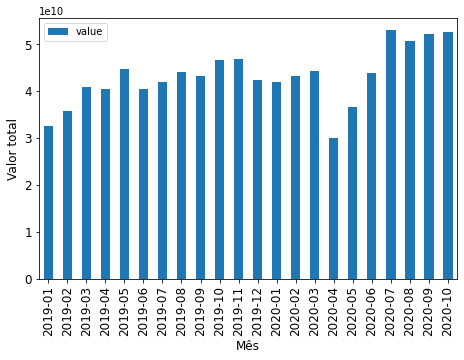
\includegraphics[scale=0.7]{images/base-de-dados-18.1-valor-mensal-total.png}
    \label{fig:pandemia:descritiva-18.1-valor-mensal-total}
    \fautor
\end{figure}

\begin{figure}[htb]
	\centering
    \caption{Quantidade total de transações por mês no período analisado}
    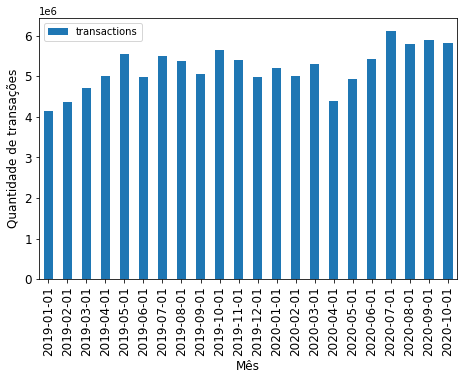
\includegraphics[scale=0.7]{images/base-de-dados-18.2-transacoes-mensal-total.png}
    \label{fig:pandemia:descritiva-18.2-transacoes-total-por-regiao}
    \fautor
\end{figure}

\begin{figure}[htb]
	\centering
    \caption{Comparação do valor total transacionado por mês entre 2019 e 2020 (Parte 4)}
    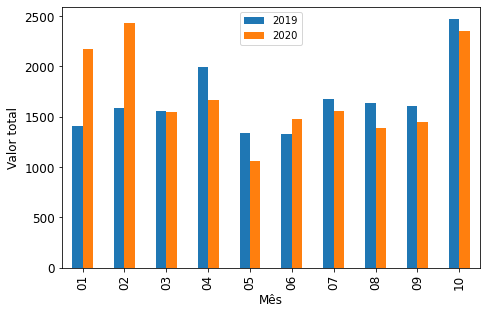
\includegraphics[scale=0.7]{images/base-de-dados-19.1-comparacao-valor-mensal-total.png}
    \label{fig:pandemia:descritiva-19.1-comparacao-valor-mensal-total}
    \fautor
\end{figure}

\begin{figure}[htb]
	\centering
    \caption{Valor total transacionado por região no período analisado}
    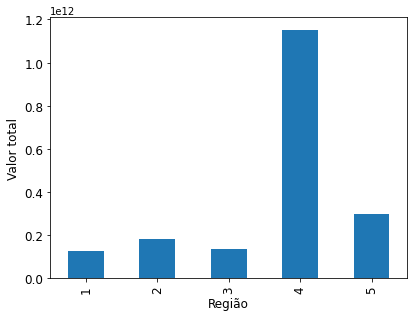
\includegraphics[scale=0.7]{images/base-de-dados-11.1-valor-total-por-regiao.png}
    \label{fig:pandemia:descritiva-11.1-valor-total-por-regiao}
    \fautor
\end{figure}

\begin{figure}[htb]
	\centering
    \caption{Quantidade total de transações por região no período analisado}
    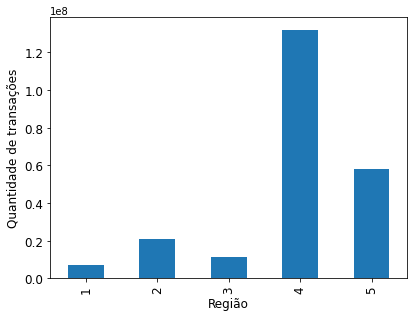
\includegraphics[scale=0.7]{images/base-de-dados-11.2-transacoes-total-por-regiao.png}
    \label{fig:pandemia:descritiva-11.2-transacoes-total-por-regiao}
    \fautor
\end{figure}

\begin{figure}[htb] 
    \centering 
    \caption{Valor mensal transacionado por região no período analisado}
    \label{fig:pandemia:descritiva-12-qtde-transacoes-mensal-por-regiao} 
    \begin{subfigure}[b]{0.45\textwidth}
        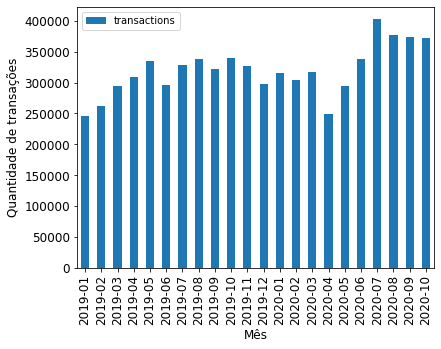
\includegraphics[scale=0.45]{images/base-de-dados-12.1-qtde-transacoes-mensal-por-regiao.png}
        \caption{Região 1}
        \label{fig:pandemia:descritiva-12.1-qtde-transacoes-mensal-por-regiao}
    \end{subfigure} ~ \quad
    \begin{subfigure}[b]{0.45\textwidth}
        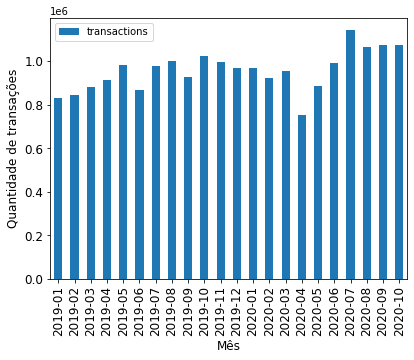
\includegraphics[scale=0.45]{images/base-de-dados-12.2-qtde-transacoes-mensal-por-regiao.png}
        \caption{Região 2}
        \label{fig:pandemia:descritiva-12.2-qtde-transacoes-mensal-por-regiao}
    \end{subfigure} ~ \\
    \begin{subfigure}[b]{0.45\textwidth}
        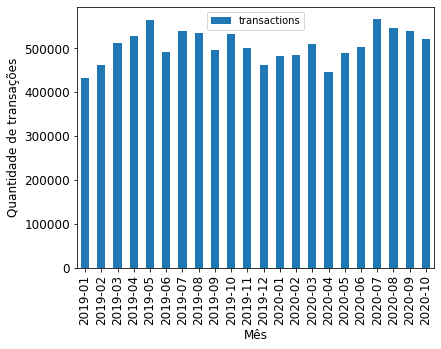
\includegraphics[scale=0.45]{images/base-de-dados-12.3-qtde-transacoes-mensal-por-regiao.png}
        \caption{Região 3}
        \label{fig:pandemia:descritiva-12.3-qtde-transacoes-mensal-por-regiao}
    \end{subfigure} ~ \quad
    \begin{subfigure}[b]{0.45\textwidth}
        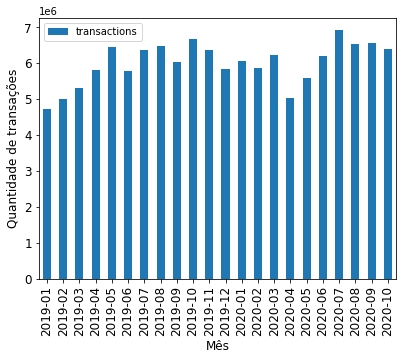
\includegraphics[scale=0.45]{images/base-de-dados-12.4-qtde-transacoes-mensal-por-regiao.png}
        \caption{Região 4}
        \label{fig:pandemia:descritiva-12.4-qtde-transacoes-mensal-por-regiao}
    \end{subfigure} ~ \\
    \begin{subfigure}[b]{0.45\textwidth} 
        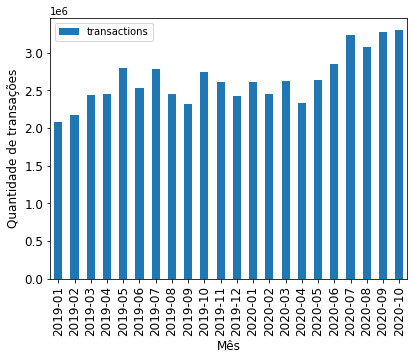
\includegraphics[scale=0.45]{images/base-de-dados-12.5-qtde-transacoes-mensal-por-regiao.png}
        \caption{Região 5}
        \label{fig:pandemia:descritiva-12.5-qtde-transacoes-mensal-por-regiao}
    \end{subfigure}
    \fautor
\end{figure}

\begin{figure}[htb] 
    \centering 
    \caption{Quantidade mensal de transações por região no período analisado}
    \label{fig:pandemia:descritiva-12-valor-mensal-por-regiao} 
    \begin{subfigure}[b]{0.45\textwidth}
        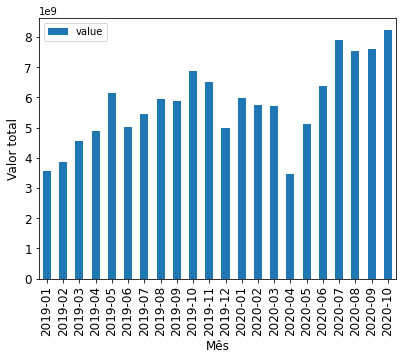
\includegraphics[scale=0.45]{images/base-de-dados-12.1-valor-mensal-por-regiao.png}
        \caption{Região 1}
        \label{fig:pandemia:descritiva-12.1-valor-mensal-por-regiao}
    \end{subfigure} ~ \quad
    \begin{subfigure}[b]{0.45\textwidth}
        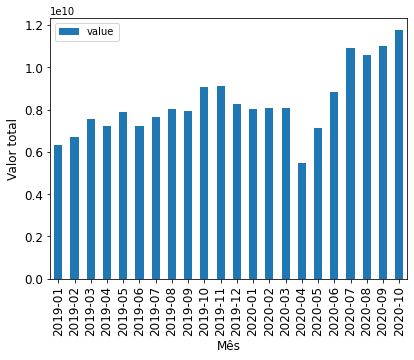
\includegraphics[scale=0.45]{images/base-de-dados-12.2-valor-mensal-por-regiao.png}
        \caption{Região 2}
        \label{fig:pandemia:descritiva-12.2-valor-mensal-por-regiao}
    \end{subfigure} ~ \\
    \begin{subfigure}[b]{0.45\textwidth}
        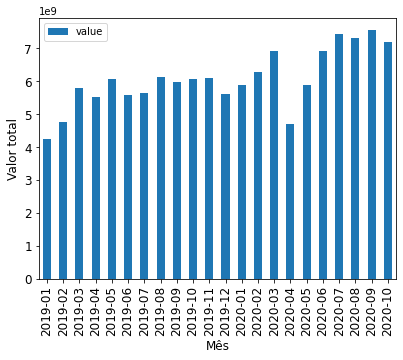
\includegraphics[scale=0.45]{images/base-de-dados-12.3-valor-mensal-por-regiao.png}
        \caption{Região 3}
        \label{fig:pandemia:descritiva-12.3-valor-mensal-por-regiao}
    \end{subfigure} ~ \quad
    \begin{subfigure}[b]{0.45\textwidth}
        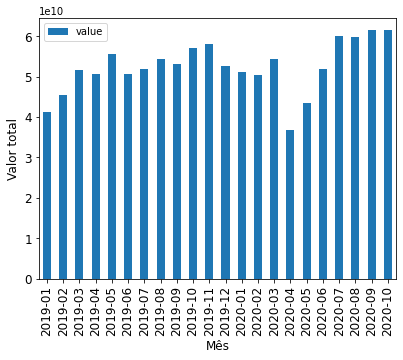
\includegraphics[scale=0.45]{images/base-de-dados-12.4-valor-mensal-por-regiao.png}
        \caption{Região 4}
        \label{fig:pandemia:descritiva-12.4-valor-mensal-por-regiao}
    \end{subfigure} ~ \\
    \begin{subfigure}[b]{0.45\textwidth} 
        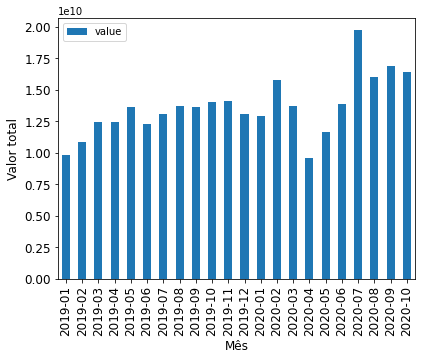
\includegraphics[scale=0.45]{images/base-de-dados-12.5-valor-mensal-por-regiao.png}
        \caption{Região 5}
        \label{fig:pandemia:descritiva-12.5-valor-mensal-por-regiao}
    \end{subfigure}
    \fautor
\end{figure}

\begin{figure}[htb] 
    \centering 
    \caption{Comparação do valor mensal transacionado por região entre 2019 e 2020}
    \label{fig:pandemia:descritiva-13-comparacao-valor-total-por-regiao} 
    \begin{subfigure}[b]{0.45\textwidth}
        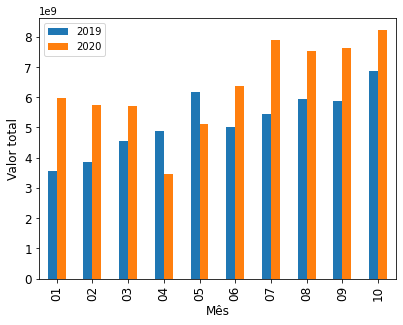
\includegraphics[scale=0.45]{images/base-de-dados-13.1-comparacao-valor-total-por-regiao.png}
        \caption{Região 1}
        \label{fig:pandemia:descritiva-13.1-comparacao-valor-total-por-regiao}
    \end{subfigure} ~ \quad
    \begin{subfigure}[b]{0.45\textwidth}
        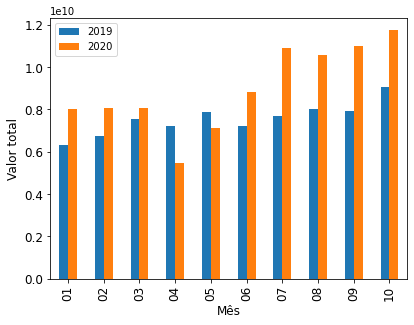
\includegraphics[scale=0.45]{images/base-de-dados-13.2-comparacao-valor-total-por-regiao.png}
        \caption{Região 2}
        \label{fig:pandemia:descritiva-13.2-comparacao-valor-total-por-regiao}
    \end{subfigure} ~ \\
    \begin{subfigure}[b]{0.45\textwidth}
        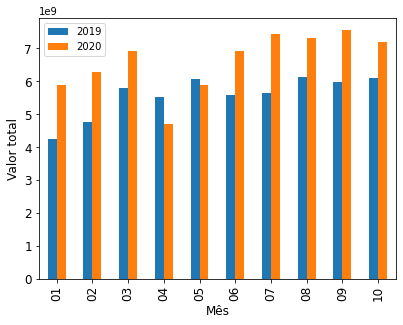
\includegraphics[scale=0.45]{images/base-de-dados-13.3-comparacao-valor-total-por-regiao.png}
        \caption{Região 3}
        \label{fig:pandemia:descritiva-13.3-comparacao-valor-total-por-regiao}
    \end{subfigure} ~ \quad
    \begin{subfigure}[b]{0.45\textwidth}
        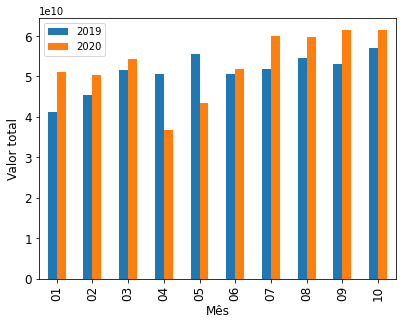
\includegraphics[scale=0.45]{images/base-de-dados-13.4-comparacao-valor-total-por-regiao.png}
        \caption{Região 4}
        \label{fig:pandemia:descritiva-13.4-comparacao-valor-total-por-regiao}
    \end{subfigure} ~ \\
    \begin{subfigure}[b]{0.45\textwidth} 
        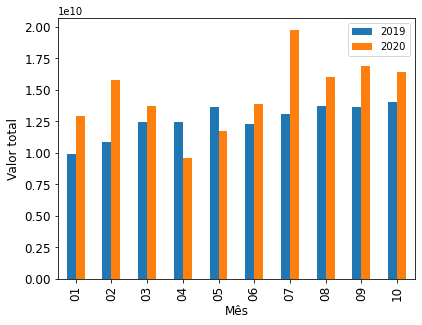
\includegraphics[scale=0.45]{images/base-de-dados-13.5-comparacao-valor-total-por-regiao.png}
        \caption{Região 5}
        \label{fig:pandemia:descritiva-13.5-comparacao-valor-total-por-regiao}
    \end{subfigure}
    \fautor
\end{figure}

\begin{figure}[htb]
	\centering
    \caption{Valor total transacionado por UF no período analisado}
    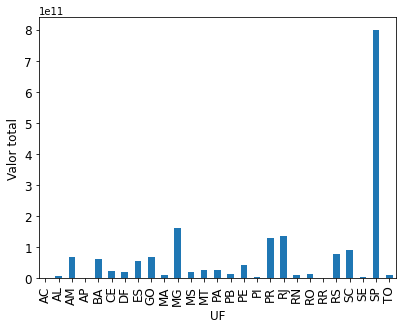
\includegraphics[scale=0.7]{images/base-de-dados-14.1-valor-total-por-uf.png}
    \label{fig:pandemia:descritiva-14.1-valor-total-por-uf}
    \fautor
\end{figure}

\begin{figure}[htb]
	\centering
    \caption{Quantidade total de transações por UF no período analisado}
    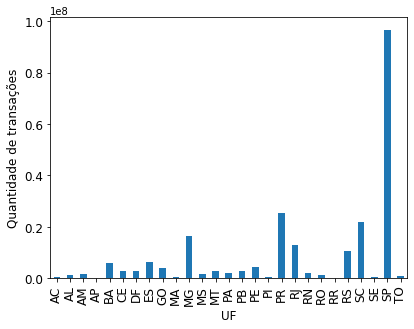
\includegraphics[scale=0.7]{images/base-de-dados-14.2-transacoes-total-por-uf.png}
    \label{fig:pandemia:descritiva-14.2-transacoes-total-por-uf}
    \fautor
\end{figure}

\begin{figure}[htb]
	\centering
    \caption{Valor total transacionado por seção no período analisado}
    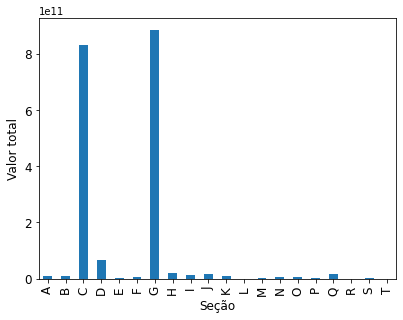
\includegraphics[scale=0.7]{images/base-de-dados-15.1-valor-total-por-secao.png}
    \label{fig:pandemia:descritiva-15.1-valor-total-por-secao}
    \fautor
\end{figure}

\begin{figure}[htb]
	\centering
    \caption{Quantidade total de transações por seção no período analisado}
    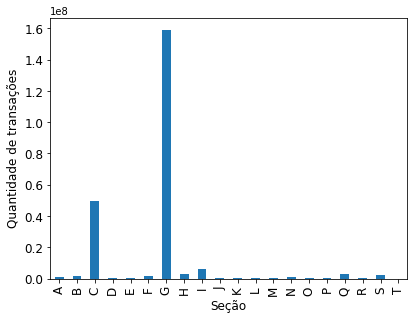
\includegraphics[scale=0.7]{images/base-de-dados-15.2-transacoes-total-por-secao.png}
    \label{fig:pandemia:descritiva-15.2-transacoes-total-por-secao}
    \fautor
\end{figure}

\begin{figure}[htb] 
    \centering 
    \caption{Valor mensal transacionado por seção no período analisado (Parte 1)}
    \label{fig:pandemia:descritiva-16.1-valor-mensal-por-secao} 
    \begin{subfigure}[b]{0.45\textwidth}
        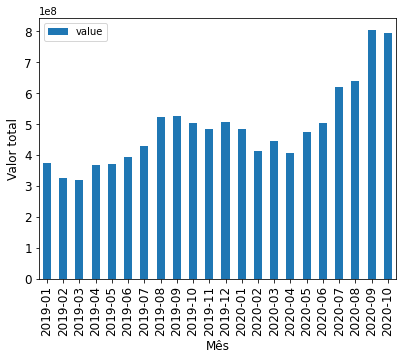
\includegraphics[scale=0.45]{images/base-de-dados-16.A-valor-mensal-por-secao.png}
        \caption{Seção A}
        \label{fig:pandemia:descritiva-16.A-valor-mensal-por-secao}
    \end{subfigure} ~ \quad
    \begin{subfigure}[b]{0.45\textwidth}
        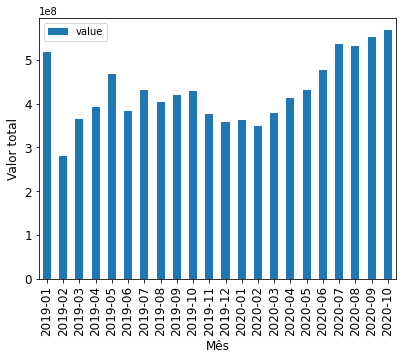
\includegraphics[scale=0.45]{images/base-de-dados-16.B-valor-mensal-por-secao.png}
        \caption{Seção B}
        \label{fig:pandemia:descritiva-16.B-valor-mensal-por-secao}
    \end{subfigure} ~ \\
    \begin{subfigure}[b]{0.45\textwidth}
        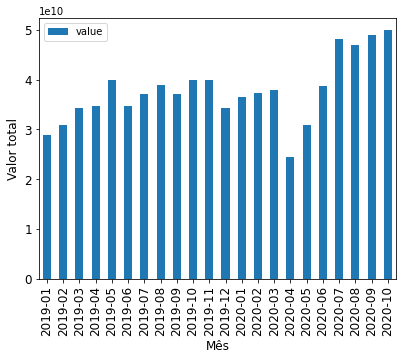
\includegraphics[scale=0.45]{images/base-de-dados-16.C-valor-mensal-por-secao.png}
        \caption{Seção C}
        \label{fig:pandemia:descritiva-16.C-valor-mensal-por-secao}
    \end{subfigure} ~ \quad
    \begin{subfigure}[b]{0.45\textwidth}
        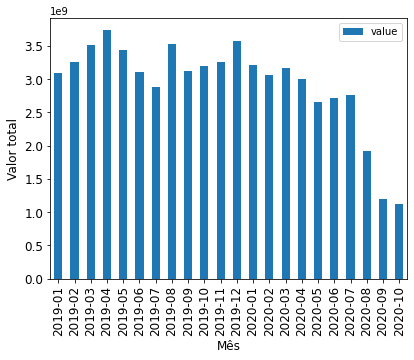
\includegraphics[scale=0.45]{images/base-de-dados-16.D-valor-mensal-por-secao.png}
        \caption{Seção D}
        \label{fig:pandemia:descritiva-16.D-valor-mensal-por-secao}
    \end{subfigure} ~ \\
    \begin{subfigure}[b]{0.45\textwidth} 
        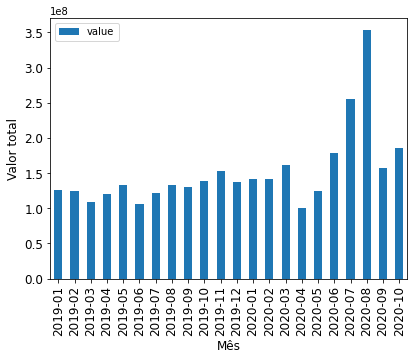
\includegraphics[scale=0.45]{images/base-de-dados-16.E-valor-mensal-por-secao.png}
        \caption{Seção E}
        \label{fig:pandemia:descritiva-16.E-valor-mensal-por-secao}
    \end{subfigure} ~ \quad
    \begin{subfigure}[b]{0.45\textwidth}
        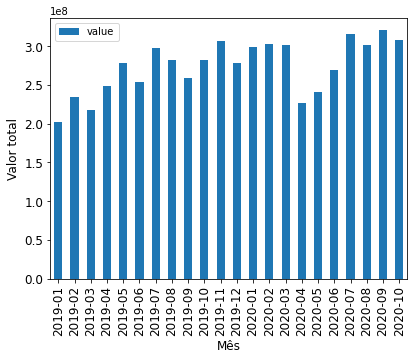
\includegraphics[scale=0.45]{images/base-de-dados-16.F-valor-mensal-por-secao.png}
        \caption{Seção F}
        \label{fig:pandemia:descritiva-16.F-valor-mensal-por-secao}
    \end{subfigure} ~ \\
    \fautor
\end{figure}

\begin{figure}[htb] 
    \centering 
    \caption{Valor mensal transacionado por seção no período analisado (Parte 2)}
    \label{fig:pandemia:descritiva-16.2-valor-mensal-por-secao} 
    \begin{subfigure}[b]{0.45\textwidth}
        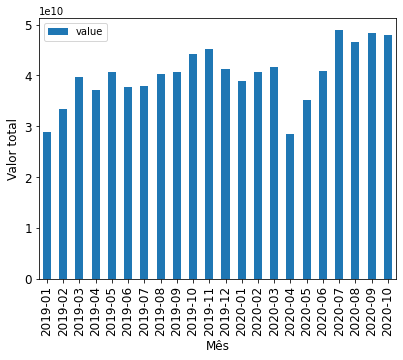
\includegraphics[scale=0.45]{images/base-de-dados-16.G-valor-mensal-por-secao.png}
        \caption{Seção G}
        \label{fig:pandemia:descritiva-16.G-valor-mensal-por-secao}
    \end{subfigure} ~ \quad
    \begin{subfigure}[b]{0.45\textwidth}
        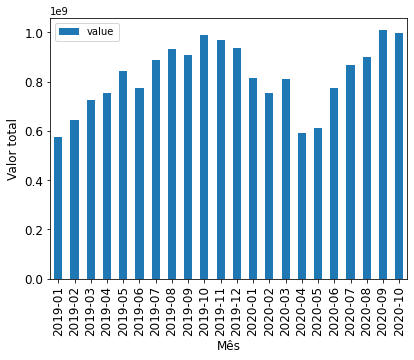
\includegraphics[scale=0.45]{images/base-de-dados-16.H-valor-mensal-por-secao.png}
        \caption{Seção H}
        \label{fig:pandemia:descritiva-16.H-valor-mensal-por-secao}
    \end{subfigure} ~ \\
    \begin{subfigure}[b]{0.45\textwidth}
        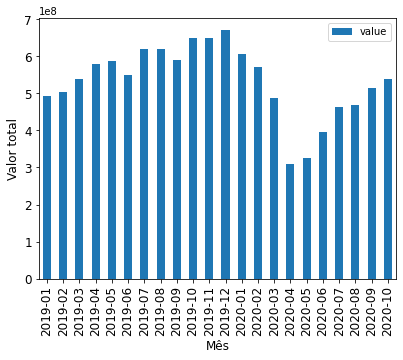
\includegraphics[scale=0.45]{images/base-de-dados-16.I-valor-mensal-por-secao.png}
        \caption{Seção I}
        \label{fig:pandemia:descritiva-16.I-valor-mensal-por-secao}
    \end{subfigure} ~ \quad
    \begin{subfigure}[b]{0.45\textwidth}
        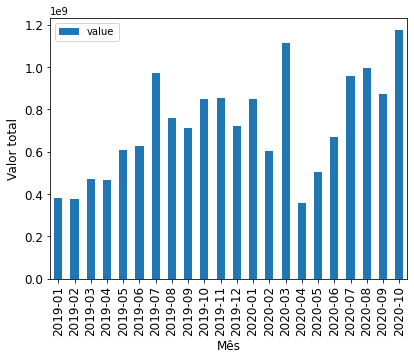
\includegraphics[scale=0.45]{images/base-de-dados-16.J-valor-mensal-por-secao.png}
        \caption{Seção J}
        \label{fig:pandemia:descritiva-16.J-valor-mensal-por-secao}
    \end{subfigure} ~ \\
    \begin{subfigure}[b]{0.45\textwidth} 
        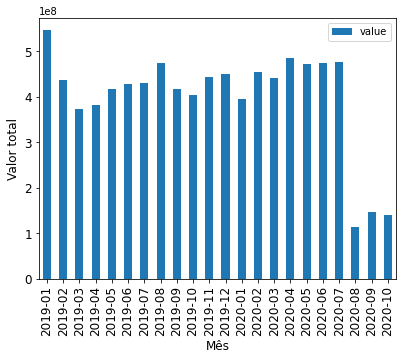
\includegraphics[scale=0.45]{images/base-de-dados-16.K-valor-mensal-por-secao.png}
        \caption{Seção K}
        \label{fig:pandemia:descritiva-16.K-valor-mensal-por-secao}
    \end{subfigure} ~ \quad
    \begin{subfigure}[b]{0.45\textwidth}
        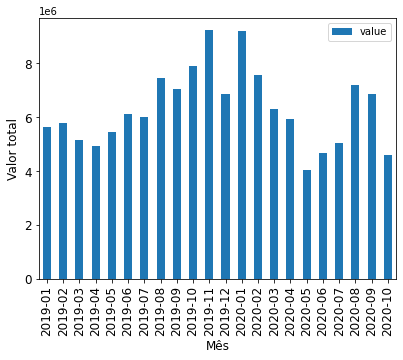
\includegraphics[scale=0.45]{images/base-de-dados-16.L-valor-mensal-por-secao.png}
        \caption{Seção L}
        \label{fig:pandemia:descritiva-16.L-valor-mensal-por-secao}
    \end{subfigure} ~ \\
    \fautor
\end{figure}

\begin{figure}[htb] 
    \centering 
    \caption{Valor mensal transacionado por seção no período analisado (Parte 3)}
    \label{fig:pandemia:descritiva-16.3-valor-mensal-por-secao} 
    \begin{subfigure}[b]{0.45\textwidth}
        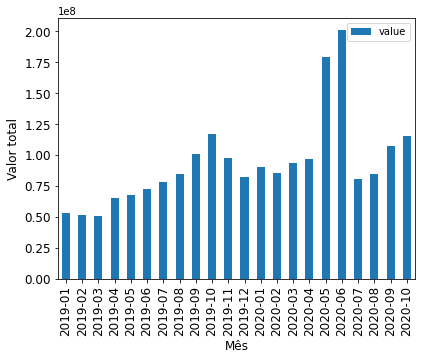
\includegraphics[scale=0.45]{images/base-de-dados-16.M-valor-mensal-por-secao.png}
        \caption{Seção M}
        \label{fig:pandemia:descritiva-16.M-valor-mensal-por-secao}
    \end{subfigure} ~ \quad
    \begin{subfigure}[b]{0.45\textwidth}
        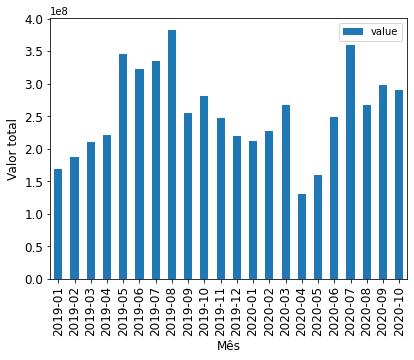
\includegraphics[scale=0.45]{images/base-de-dados-16.N-valor-mensal-por-secao.png}
        \caption{Seção N}
        \label{fig:pandemia:descritiva-16.N-valor-mensal-por-secao}
    \end{subfigure} ~ \\
    \begin{subfigure}[b]{0.45\textwidth}
        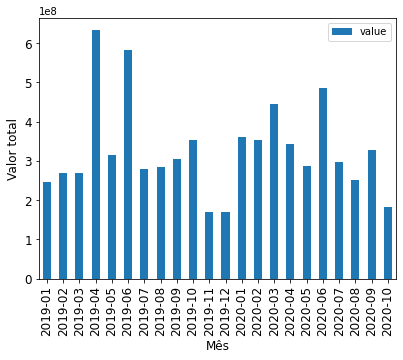
\includegraphics[scale=0.45]{images/base-de-dados-16.O-valor-mensal-por-secao.png}
        \caption{Seção O}
        \label{fig:pandemia:descritiva-16.O-valor-mensal-por-secao}
    \end{subfigure} ~ \quad
    \begin{subfigure}[b]{0.45\textwidth}
        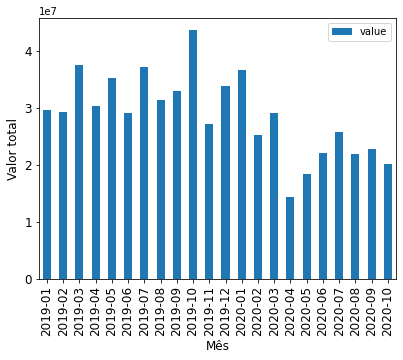
\includegraphics[scale=0.45]{images/base-de-dados-16.P-valor-mensal-por-secao.png}
        \caption{Seção P}
        \label{fig:pandemia:descritiva-16.P-valor-mensal-por-secao}
    \end{subfigure} ~ \\
    \begin{subfigure}[b]{0.45\textwidth} 
        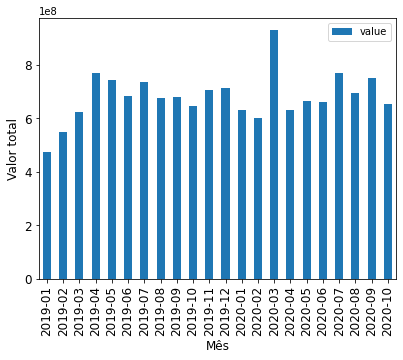
\includegraphics[scale=0.45]{images/base-de-dados-16.Q-valor-mensal-por-secao.png}
        \caption{Seção Q}
        \label{fig:pandemia:descritiva-16.Q-valor-mensal-por-secao}
    \end{subfigure} ~ \quad
    \begin{subfigure}[b]{0.45\textwidth}
        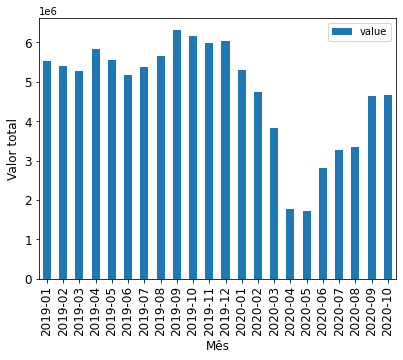
\includegraphics[scale=0.45]{images/base-de-dados-16.R-valor-mensal-por-secao.png}
        \caption{Seção R}
        \label{fig:pandemia:descritiva-16.R-valor-mensal-por-secao}
    \end{subfigure} ~ \\
    \fautor
\end{figure}

\begin{figure}[htb] 
    \centering 
    \caption{Valor mensal transacionado por seção no período analisado (Parte 4)}
    \label{fig:pandemia:descritiva-16.4-valor-mensal-por-secao} 
    \begin{subfigure}[b]{0.45\textwidth}
        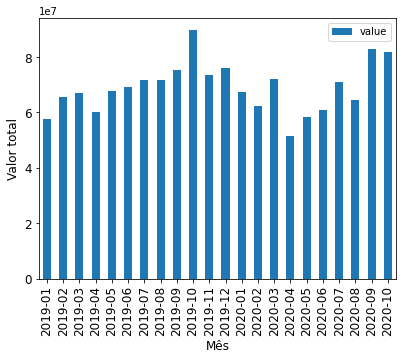
\includegraphics[scale=0.45]{images/base-de-dados-16.S-valor-mensal-por-secao.png}
        \caption{Seção S}
        \label{fig:pandemia:descritiva-16.S-valor-mensal-por-secao}
    \end{subfigure} ~ \quad
    \begin{subfigure}[b]{0.45\textwidth}
        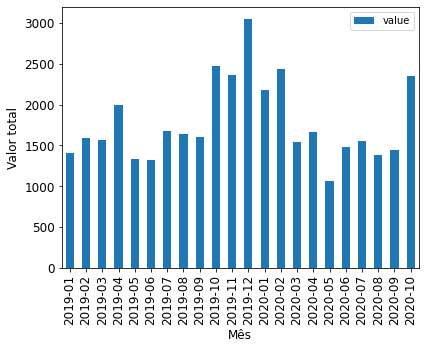
\includegraphics[scale=0.45]{images/base-de-dados-16.T-valor-mensal-por-secao.png}
        \caption{Seção T}
        \label{fig:pandemia:descritiva-16.T-valor-mensal-por-secao}
    \end{subfigure}
    \fautor
\end{figure}

\begin{figure}[htb] 
    \centering 
    \caption{Comparação do valor mensal transacionado por seção entre 2019 e 2020 (Parte 1)}
    \label{fig:pandemia:descritiva-17.1-comparacao-valor-total-por-secao} 
    \begin{subfigure}[b]{0.45\textwidth}
        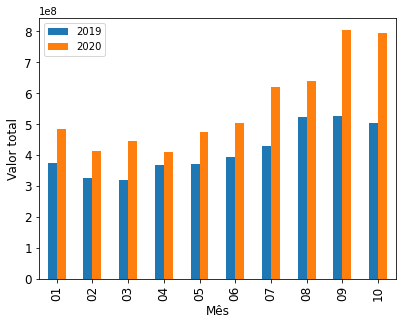
\includegraphics[scale=0.45]{images/base-de-dados-17.A-comparacao-valor-total-por-secao.png}
        \caption{Seção A}
        \label{fig:pandemia:descritiva-17.A-comparacao-valor-total-por-secao}
    \end{subfigure} ~ \quad
    \begin{subfigure}[b]{0.45\textwidth}
        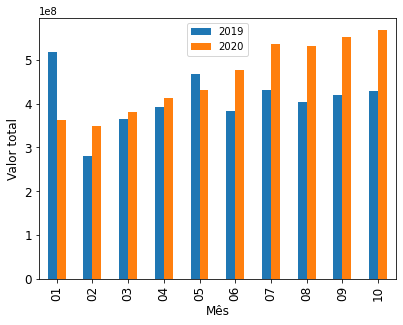
\includegraphics[scale=0.45]{images/base-de-dados-17.B-comparacao-valor-total-por-secao.png}
        \caption{Seção B}
        \label{fig:pandemia:descritiva-17.B-comparacao-valor-total-por-secao}
    \end{subfigure} ~ \\
    \begin{subfigure}[b]{0.45\textwidth}
        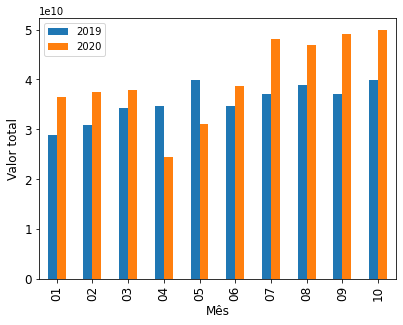
\includegraphics[scale=0.45]{images/base-de-dados-17.C-comparacao-valor-total-por-secao.png}
        \caption{Seção C}
        \label{fig:pandemia:descritiva-17.C-comparacao-valor-total-por-secao}
    \end{subfigure} ~ \quad
    \begin{subfigure}[b]{0.45\textwidth}
        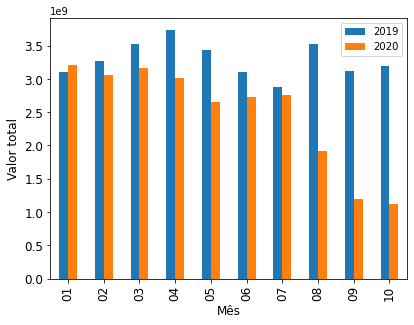
\includegraphics[scale=0.45]{images/base-de-dados-17.D-comparacao-valor-total-por-secao.png}
        \caption{Seção D}
        \label{fig:pandemia:descritiva-17.D-comparacao-valor-total-por-secao}
    \end{subfigure} ~ \\
    \begin{subfigure}[b]{0.45\textwidth} 
        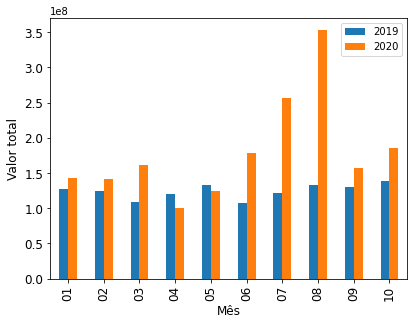
\includegraphics[scale=0.45]{images/base-de-dados-17.E-comparacao-valor-total-por-secao.png}
        \caption{Seção E}
        \label{fig:pandemia:descritiva-17.E-comparacao-valor-total-por-secao}
    \end{subfigure} ~ \quad
    \begin{subfigure}[b]{0.45\textwidth}
        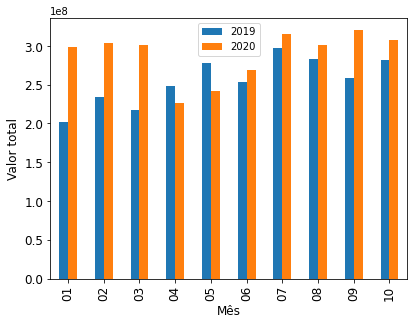
\includegraphics[scale=0.45]{images/base-de-dados-17.F-comparacao-valor-total-por-secao.png}
        \caption{Seção F}
        \label{fig:pandemia:descritiva-17.F-comparacao-valor-total-por-secao}
    \end{subfigure} ~ \\
    \fautor
\end{figure}

\begin{figure}[htb] 
    \centering 
    \caption{Comparação do valor mensal transacionado por seção entre 2019 e 2020 (Parte 2)}
    \label{fig:pandemia:descritiva-17.2-comparacao-valor-total-por-secao} 
    \begin{subfigure}[b]{0.45\textwidth}
        \includegraphics[scale=0.45]{images/base-de-dados-17.G-comparacao-valor-total-por-secao.png}
        \caption{Seção G}
        \label{fig:pandemia:descritiva-17.G-comparacao-valor-total-por-secao}
    \end{subfigure} ~ \quad
    \begin{subfigure}[b]{0.45\textwidth}
        \includegraphics[scale=0.45]{images/base-de-dados-17.H-comparacao-valor-total-por-secao.png}
        \caption{Seção H}
        \label{fig:pandemia:descritiva-17.H-comparacao-valor-total-por-secao}
    \end{subfigure} ~ \\
    \begin{subfigure}[b]{0.45\textwidth}
        \includegraphics[scale=0.45]{images/base-de-dados-17.I-comparacao-valor-total-por-secao.png}
        \caption{Seção I}
        \label{fig:pandemia:descritiva-17.I-comparacao-valor-total-por-secao}
    \end{subfigure} ~ \quad
    \begin{subfigure}[b]{0.45\textwidth}
        \includegraphics[scale=0.45]{images/base-de-dados-17.J-comparacao-valor-total-por-secao.png}
        \caption{Seção J}
        \label{fig:pandemia:descritiva-17.J-comparacao-valor-total-por-secao}
    \end{subfigure} ~ \\
    \begin{subfigure}[b]{0.45\textwidth} 
        \includegraphics[scale=0.45]{images/base-de-dados-17.K-comparacao-valor-total-por-secao.png}
        \caption{Seção K}
        \label{fig:pandemia:descritiva-17.K-comparacao-valor-total-por-secao}
    \end{subfigure} ~ \quad
    \begin{subfigure}[b]{0.45\textwidth}
        \includegraphics[scale=0.45]{images/base-de-dados-17.L-comparacao-valor-total-por-secao.png}
        \caption{Seção L}
        \label{fig:pandemia:descritiva-17.L-comparacao-valor-total-por-secao}
    \end{subfigure} ~ \\
    \fautor
\end{figure}

\begin{figure}[htb] 
    \centering 
    \caption{Comparação do valor mensal transacionado por seção entre 2019 e 2020 (Parte 3)}
    \label{fig:pandemia:descritiva-17.3-comparacao-valor-total-por-secao} 
    \begin{subfigure}[b]{0.45\textwidth}
        \includegraphics[scale=0.45]{images/base-de-dados-17.M-comparacao-valor-total-por-secao.png}
        \caption{Seção M}
        \label{fig:pandemia:descritiva-17.M-comparacao-valor-total-por-secao}
    \end{subfigure} ~ \quad
    \begin{subfigure}[b]{0.45\textwidth}
        \includegraphics[scale=0.45]{images/base-de-dados-17.N-comparacao-valor-total-por-secao.png}
        \caption{Seção N}
        \label{fig:pandemia:descritiva-17.N-comparacao-valor-total-por-secao}
    \end{subfigure} ~ \\
    \begin{subfigure}[b]{0.45\textwidth}
        \includegraphics[scale=0.45]{images/base-de-dados-17.O-comparacao-valor-total-por-secao.png}
        \caption{Seção O}
        \label{fig:pandemia:descritiva-17.O-comparacao-valor-total-por-secao}
    \end{subfigure} ~ \quad
    \begin{subfigure}[b]{0.45\textwidth}
        \includegraphics[scale=0.45]{images/base-de-dados-17.P-comparacao-valor-total-por-secao.png}
        \caption{Seção P}
        \label{fig:pandemia:descritiva-17.P-comparacao-valor-total-por-secao}
    \end{subfigure} ~ \\
    \begin{subfigure}[b]{0.45\textwidth} 
        \includegraphics[scale=0.45]{images/base-de-dados-17.Q-comparacao-valor-total-por-secao.png}
        \caption{Seção Q}
        \label{fig:pandemia:descritiva-17.Q-comparacao-valor-total-por-secao}
    \end{subfigure} ~ \quad
    \begin{subfigure}[b]{0.45\textwidth}
        \includegraphics[scale=0.45]{images/base-de-dados-17.R-comparacao-valor-total-por-secao.png}
        \caption{Seção R}
        \label{fig:pandemia:descritiva-17.R-comparacao-valor-total-por-secao}
    \end{subfigure} ~ \\
    \fautor
\end{figure}

\begin{figure}[htb] 
    \centering 
    \caption{Comparação do valor mensal transacionado por seção entre 2019 e 2020 (Parte 4)}
    \label{fig:pandemia:descritiva-17.4-comparacao-valor-total-por-secao} 
    \begin{subfigure}[b]{0.45\textwidth}
        \includegraphics[scale=0.45]{images/base-de-dados-17.S-comparacao-valor-total-por-secao.png}
        \caption{Seção S}
        \label{fig:pandemia:descritiva-17.S-comparacao-valor-total-por-secao}
    \end{subfigure} ~ \quad
    \begin{subfigure}[b]{0.45\textwidth}
        \includegraphics[scale=0.45]{images/base-de-dados-17.T-comparacao-valor-total-por-secao.png}
        \caption{Seção T}
        \label{fig:pandemia:descritiva-17.T-comparacao-valor-total-por-secao}
    \end{subfigure}
    \fautor
\end{figure}
